\begin{figure}[H]
\centering
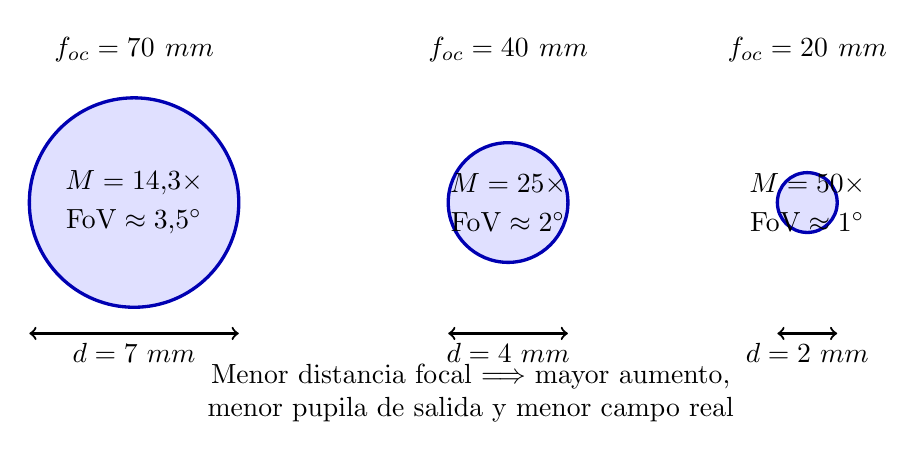
\begin{tikzpicture}[scale=0.95]
  \foreach \x/\r/\diam/\foc/\mag/\campo in
    {0/1.40/7/70/{14{,}3}/{3{,}5^\circ},
     5/0.80/4/40/25/{2^\circ},
     9/0.40/2/20/50/{1^\circ}}{
    \fill[blue!12] (\x,0) circle (\r);
    \draw[blue!70!black,very thick] (\x,0) circle (\r);
    \draw[<->,thick] (\x-\r,-1.75) -- (\x+\r,-1.75)
      node[midway,below] {$d=\diam~\text{mm}$};
    \node[font=\bfseries] at (\x,2.05) {$f_{\text{oc}}=\foc~\text{mm}$};
    \node[align=center] at (\x,0)
      {$M=\mag\times$\\[2pt]$\mathrm{FoV}\approx\campo$};
  }
  \node[align=center] at (4.5,-2.55)
    {Menor distancia focal $\Longrightarrow$ mayor aumento,\\
     menor pupila de salida y menor campo real};
\end{tikzpicture}
\caption{Comparación de las configuraciones visuales del telescopio. Los círculos representan las pupilas de salida a escala relativa.}
\end{figure}